\graphicspath{{Pics/combi/graph/}}


\newpage\section{Graph Theory}


	\begin{take_note*}{Turning grids into graphs}
		\begin{itemize}
			\item One common way to turn a grid into graphs is to create a bipartite graph between the columns and rows such that $ c_i $ and $ r_j $ are connected iff $ (i, j) $ is marked. This way we can find cycles alternating row and column.
			
			\item Creating a bipartite graph between all rows and columns and particular objects. This helps to prove matching. 
		\end{itemize}
	\end{take_note*}

	\faka



	\lem{Bipartite Graph Criteria}{Any graph having only even cycles are \emph{Bipartite}.}\label{lemma:bipartite_graph}\index{Bipartite}

		\begin{multicols}{3}
			\begin{enumerate}[wide=0em, label=\arabic*, itemsep=0pt, parsep=0pt, font=\footnotesize\bfseries]

				\iref{problem:bipartite_graph_1}{AoPS}{}
				\iref{problem:bipartite_graph_2}{ISL 2004 C3}{}
				\iref{problem:bipartite_graph_3}{Problem}{}
				\iref{problem:bipartite_graph_4}{Problem}{}
			\end{enumerate}
		\end{multicols}


	\theo{http://www.ams.org/samplings/feature-column/fcarc-eulers-formula}{Euler's Polyhedron Formula}{
		\begin{itemize}[wide=0pt]
			\itemsep-1.5em
			\item For any polyhedron with $ E, V, F $ edges, vertices's and faces resp. the following relation holds \[V+F=E+2\]\label{lemma:planar_graph_polyhedron}
			\item In a planar graph with $ V $ vertices, $ E $ edges and $ C $ cycles, the following condition is always satisfied: \[V-E+C=1\]\label{theorem:planar_graph_theorem}
		\end{itemize}\index{Polyhedron Formula}}
	

	
	
	\lem{Criteria of partitioning a graph into disconnected sub-graphs}{If there exist no three vertices, $ u,v,w $ that $ uv\in E(G) $ also $ uw, vw\in E(G) $, the graph can be partitioned into equivalence classes based on their non-neighbors.\index{Non-Neighbor Equivalence Class}}\label{lemma:criteria_of_partition_equiv}
	
		
	
	\prob{https://artofproblemsolving.com/community/c6h1063060p4609322}{China TST 2015 T1 D2 P3}{E}{There are some players in a Ping Pong tournament, where every $2$ players play with each other at most once. Given:
		\vspace{-.9em}
		\begin{enumerate}
			\itemsep-.3em
			\item Each player wins against at least $a$ players, and loses to at least $b$ players. ($a,b\geq 1$)
			\item For any two players $A,B$, there exist some players $P_1,...,P_k$ ($k\geq 2$) (where $P_1=A$,$P_k=B$), such that $P_i$ wins against $P_{i+1}$ ($i=1,2...,k-1$)
		\end{enumerate}
		\vspace{-.9em}
	Prove that there exist $a+b+1$ distinct players $Q_1,...Q_{a+b+1}$, such that $Q_i$ wins against $Q_{i+1}$ ($i=1,...,a+b$).\index{Extremal!Longest Path!ChTST 2015 P3}}

		\rem{Typical largest path, some workaround with given constraints problem.}

		\solu{Take the largest path starting from $ a_1 $ to $ a_n $. 
			\begin{solution_def}
				Assume that $ n\le a+b $. Since this is the largest path, $ a $ edges coming out of $ a_n $ are all in $ S=\{a_1, a_2, \dots a_n\} $, and $ b $ edges going in $ a_1 $ are all in $ S $. Let $ S_1 $ be the set of vertices that $ a_n $ wins against, and $ S_2 $ be the set of vertices that $ a_1 $ loses against. Moreover, let $ a_l $ be the smallest element of $ S_1 $, and $ a_{n-k} $ be the largest element of $ S_2 $ (smallest means leftmost in the part, and largest means rightmost).\\
				
				Let $ S'=\{a_l, a_{l+1}, \dots a_{n-k-1}, a_{n-k}\} $. Since $ n\le a+b $, we have $ S'\ne \varnothing $. \\
				
				We also define:
					\[ S_1'=\{a_i\mid a_i \text{ defeats } a_{i+1} \text{ where } a_{i+1} \in S_1\cap S' \}\]
					\[S_2'=\{a_i\mid a_{i-1} \text{ defeats } a_{i} \text{ where } a_{i-1} \in S_2\cap S'\}\]
			\end{solution_def}
			\figdf{.4}{China_TST_2015_T1_D2_P3_1}{}
		Now, note that for any $ x\in S_2' $, $ y\in S_1' $, there is a path between $ x, y $ with $ n $ vertices. So for all $ x\in S_2' $, there does not exist a vertex outside of $ S $ that defeats $ x $. And for all $ y\in S_1' $, there doesn't exist a vertex outside of $ S $ that loses to $ y $, because of the maximality of $ n $. \\
		
		We show that, $ S_1'\cap S_2' \ne \varnothing $. Then there would exist a vertex that doesn't have any edge outside of $ S $, meaning it has at least $ a+b $ games inside $ S $, proving the result.\\ 
		
		We have, $ S_1', S_2' \subset S'\cup\{a_{l-1}, a_{n-k+1}\} $. We have, 
			\begin{align*}
				|S_1'| &\ge a-k+2\quad [\because a_n \text{ has at most } k-2 \text{ vertices in } \{a_{n-k+1}, \dots a_n\}]\\
				|S_2'| &\ge b-l+3
			\end{align*}
		But $ |S'|=n-(l-1)-(k)+2 \le a+b-l-k+3 < |S_1'|+|S_2'| $. So $ S_1'\cap S_2' \ne \varnothing $, and we are done.}
		
		
		
	\prob{https://artofproblemsolving.com/community/c6h35315p220222}{ARO 2005 P10.8}{E}{A white plane is partitioned in to cells (in a usual way). A finite number of cells are coloured black. Each black cell has an even (0, 2 or 4) number of adjacent (by the side) white cells. Prove that one may colour each white cell in green or red such that every black cell will have equal number of red and green adjacent cells.\index{Graph!Grid $ \to $ Graph!ARO 2005 P10.8}\index{Graph!Bipartite!ARO 2005 P10.8}}
		
		\solu{First we join the white cells like this:
			\figdf{.8}{ARO_2005_P10_8}{}
			Now, notice that the plane have been divided into some cycles (a black cell that has no adjacent black cells is a cycle itself). So we can color the plane blue and yellow in a way that no region has the same color as its neighbors. We can do this because at any junction, there are an even number of regions connected because of the problem condition.\\
			
			Now we focus on our graph that we created connected the white cells. Take any cycle on it. If we have a ``slanted'' edge, then both of the nodes are inside a region of either blue or yellow. But in a ``straight'' edge, the two nodes are in different colored region.\\
			
			We know that there are an even number of slanted edges, which is trivial to prove (using the fact that any cycle on a grid system has even number of nodes, and on these cycles, most of the edges (the straight ones) have even lenght, but only the slanted one has odd lenghts on the sides). It is also easy to see that there are an even number of straight edges, because of going in and out of the regions of a fixed color.\\
			
			So our cycle has an even number of nodes and thus bipartite. We can color the graph with two colors, so that along each edge, the two nodes are of different color.}
		
		\rem{There is a simple coloring using this solution. After we color the regions of the plane with blue and yellow, we number each column with integers. Then on the odd numbered columns, we color all the white cells that are in yellow region green and blue region red. And on the even numbered columns, we do the opposite. It is easy to check that this coloring works using the graph we created before.}
		
			
			
	\prob{https://atcoder.jp/contests/agc033/tasks/agc033_c}{AtCoder GC033 C}{E}{Takahashi and Aoki will play a game on a tree. The tree has $ N $ vertices numbered $ 1 $ to $ N $, and the $ i $-th of the $ N-1 $ edges connects Vertex $ a_i $ and Vertex $ b_i $
		
	At the beginning of the game, each vertex contains a coin. Starting from Takahashi, he and Aoki will alternately perform the following operation:
		
		\begin{itemize}
			\item Choose a vertex $ v $ that contains one or more coins, and remove all the coins from $ v $.
			\item Then, move each coin remaining on the tree to the vertex that is nearest to $ v $	among the adjacent vertices of the coin's current vertex.
		\end{itemize}
		
	The player who becomes unable to play, loses the game. That is, the player who takes his turn when there is no coin remaining on the tree, loses the game. Determine the winner of the game when both players play optimally.\index{Extremal!Longest Path!AtCoder GC033 C}\index{Invariant!Monovariant!AtCoder GC033 C}}

	\solu{First transform the game by removing the idea of coins, and replacing it with deleting vertices. Now, notice that the longest path in this tree (i.e. the diameter) strictly decreases by $ 1 $ or $ 2 $ each turn depending on the move. So it's just a basic predetermined game.}
		
		
	\prob{https://artofproblemsolving.com/community/c6h514375p2889828}{ARO 1999 P9.8}{M}{There are $2000$ components in a circuit, every two of which were initially joined by a wire. The hooligans Vasya and Petya cut the wires one after another. Vasya, who starts, cuts one wire on his turn, while Petya cuts one or three. The hooligan who cuts the last wire from some component loses. Who has the winning strategy?\index{Algorithm!Copycat!ARO 1999 P9.8}}
	
		\solu{[Copycat]
		The P-Hooligan Petya has a winning strategy, for he can be follow the old cunning trick of never losing. How does he do it?
			
		He starts by secretly partitioning the vertices in two $ 1000 $ degree subsets. He calls them $ A= \{a_1, a_2\dots a_{1000}\} $ and $ B=\{b_1, b_2 \dots b_{1000}\} $. He then connects $ a_i $ with $ b_i $ with an edge with an invisible marker that only he can see. 
		
		Now the game begins. Petya copies Vasyas moves following these rules:
			\begin{enumerate}
				\itemsep.5em
				\item If Vasya removes an edge $ a_i$ -- $a_j $, where $ i\ne j $, then Patya removes the edges $ a_i$ -- $b_j,\ a_j$ -- $b_i$ and $ b_i$ -- $b_j $.
				\item If Vasya removes $a_j$ -- $b_i$, where $ i\ne j $, then Patya removes the other three edges from the above rule.
				\item If Vasya removes $ a_i $--$ b_i $, then Patya looks for another $ b_j $, such that $ a_i $--$ b_j $ exists. Then by the symmetry so far maintanined, $ a_j $--$ b_i $ and $ a_j $--$ b_j $ exist too. And Patya can remove $ a_j$--$ b_j $, and swap the names of $ b_j $ and $ b_i $. 
				
				But if he can't, then that would mean after Vasya's move $ a_i $ would become isolated, and Patya would win. 
			\end{enumerate}
		It is easy to see that the above moves are possible since Patya is always maintaining symmetry between $ A, B $. So he can't move means Vasya has already disconnected one of the vertices.}
	
	
		\rem{The case with $ 4 $ vertices and $ 6 $ vertices give an idea to copy the opponent's moves.}
	
	
	
	\prob{https://artofproblemsolving.com/community/c6h17455p119177}{ISL 2001 C3}{E}{Define a $ k $-clique to be a set of $ k $ people such that every pair of them are acquainted with each other. At a certain party, every pair of $ 3 $-cliques has at least one person in common, and there are no $ 5 $-cliques. Prove that there are two or fewer people at the party whose departure leaves no $ 3 $-clique remaining.\index{Extremal!Object!ISL 2001 C3}}\label{problem:extreme_object_16}
	
		\solu{Casework with the point where most of the triangles are joined.}
		
		
	\prob{https://artofproblemsolving.com/community/c6h1441121p8200413}{ARO 2017 P9.1}{E}{In a country some cities are connected by one-way flights (there is at most one flight between two cities). City $ A $ is called ``available" from city $ B $, if there is a flight from $ B $ to $ A $, maybe with some transits. It is known, that for every $ 2 $ cities $ P $ and $ Q $, there exists a city $ R $, such that $ P $ and $ Q $ are both available from $ R $. Prove, that exist city $ A $, such that every city is available from $ A $.\index{Induction!Classic!ARO 2017 P9.1}}\label{problem:induction_type1_3}
	
		\solu{Basic induction exercise.}
	
	
	\prob{https://artofproblemsolving.com/community/c6h446932}{Turkey National MO 2002 P3}{}{Graph Airlines $ (GA)$ operates flights between some of the cities of the Republic of Graphia. There are at least three $ GA$ flights from each city, and it is possible to travel from any city in Graphia to any city in Graphia using $ GA$ flights. $ GA$ decides to discontinue some of its flights. Show that this can be done in such a way that it is still possible to travel between any two cities using $ GA$ flights, yet at least $ 2/9$ of the cities have only one flight.}
	
	
	
	
	
	
	
	
	
	
	\subsection{Counting in Graph}

\lem{Average of Degrees}{In a graph $ G $ with $ n $ vertexes, let $ E $ be the set of all edges. Assign an integer $ f_i $ to every vertex $ v_i $ such that $ f_i $ equals to the everage degree of the neighbors of $ v_i $. We have, \[ \sum_{i=1}^{n} f_i \geq 2|E| \] }\label{lemma:graph_lemma_1}


\lem{}{In a graph $ G $ with $ n $ vertexes, let $ E $ be the set of all edges. Assign an integer $ g_i $ to every vertex $ v_i $ such that $ g_i $ equals to the maximum degree among its neighbors. We have, \[ \sum_{i=1}^{n} g_i \geq 2|E| \] }


\prob{https://artofproblemsolving.com/community/c6h568277p3332307}{USA TST 2014 P3}{H}{Let $n$ be an even positive integer, and let $G$ be an $n$-vertex graph with exactly $\tfrac{n^2}{4}$ edges, where there are no loops or multiple edges (each unordered pair of distinct vertices is joined by either 0 or 1 edge). An unordered pair of distinct vertices $\{x,y\}$ is said to be amicable if they have a common neighbor (there is a vertex $z$ such that $xz$ and $yz$ are both edges). Prove that $G$ has at least $2\textstyle\binom{n/2}{2}$ pairs of vertices which are amicable.}

\solu{Define friendship in a different way, bounding below, keeping in mind the equality case. Then using the previous lemma.}


\begin{minipage}{.6\linewidth}
    \theo{https://en.wikipedia.org/wiki/Turan's_theorem}
    {Turan's theorem}{
        Let $ G $ be any graph with $ n $ vertices, such that $ G $ is $ K_{r+1} $
        -free. Then $ G $ is the ``Turán's Graph'' and is a complete $ r $ partite
        graph. And the number of edges in $ G $ is at most 

        \[\frac {r-1}{r}\cdot \frac {n^{2}}{2}=\left(1-\frac {1}{r}\right)\cdot
        \frac {n^{2}}{2}\]

        A special case of Turán's theorem for $ n=2 $ is the \textbf{Mantel's
        Theorem}. It states that the maximal triangle free graph is a complete
        bipartite graph with at most $ \left\lfloor\dfrac{n^2}{4}\right\rfloor $
        edges.
    }
\end{minipage}\hfill%
\begin{minipage}{.37\linewidth}
\figdf{.9}{Turan_13-4}{Turán's Graph}
\end{minipage}

\vspace{1em}


\proof{We need to prove that the maximal graph is the $ r $ partite one, and the rest will follow. We can directly try to prove that this graph is $ r $ colorable, but that is quite troublesome. Instead, we try to show that, we can partition the vertices of $ G $ into equivalence classes based on their non-neighbors. Since this is imply the former. So we need to prove that \hrf{lemma:criteria_of_partition_equiv}{this} holds for this graph.\\ 

The way it is done is quite interesting. We need to show that if the criteria doesn't hold in this graph, then this graph is not the maximal graph. How are we going to do that? We compare the degrees of $ u, w $, and replace either $ u $ by $ w $ or $ w $ by $ u $ to get a graph with more edges and without the nasty situation.}



\prob{}{}{E}{$ 155 $ birds $ P_1, P_2, \dots, P_{155} $ are sitting down no the boundary of a circle $ C $. Two birds $ P_i, P_j $ are mutually visible if the angle at the center of their cord, $ m(P_iP_j)\le 10^\circ $. Find the smallest number of mutually visible pairs of birds.}


\prob{}{}{E}{For a pair $ A = (x_1, y_1) $ and $ B = (x_2, y_2) $ of points on the coordinate plane, let $ d(A, B)  = |x_1 - x_2| + |y_1 - y_2|$. We call a pair $ (A,B) $  of unordered points harmonic if $ 1<d(A,B)\le 2 $. Determine the maximum number of harminc pairs among $ 100 $ points in the plane.}





\prob{www.hehe.com}{Swell coloring}{E}{Let $ K_n $ denote the complete graph on $ n $ vertices, that is, the graph with $ n $ vertices's such that every pair of vertices's is connected by an edge. A swell coloring of $ K_n $ is an assignment of a color to each of the edges such that the edges of any triangle are either all of distinct colors or all the same color. Further, more than one color must be used in total (otherwise trivially if all edges are the same color we would have a swell coloring). Show that if $ K_n $ can be swell colored with $ k $ colors, then $ k \geq \sqrt{n} + 1 $.}\label{problem:forget_and_focus_5}

\solu{Concentrate on only one vertex.}



\prob{www.hehe.com}{Belarus 2001}{MH}{Given $ n $ people, any two are either friends or enemies, and friendship and enmity are mutual. I want to distribute hats to	them, in such a way that any two friends possess a hat of the same color but no two enemies possess a hat of the same color. Each person can receive multiple hats. What is the minimum number of colors required to always guarantee that I can do this?}\label{problem:extremal_case_whole_6}

\solu{In this problem, finding the worst case is a big help, because once the answer is guessed, the things become really clear.}



\prob{https://artofproblemsolving.com/community/c6h1468154p8509521}{ELMO 2017 P5}{M (8/10)}{The edges of $ K_{2017} $ are each labeled with $ 1, 2 $ or $ 3 $ such that any triangle has sum of labels at least $ 5. $ Determine the minimum possible average of all labels. (Here $ K_{2017} $ is defined as the complete graph on 2017 vertices's, with an edge between every pair of vertices's.)}\label{problem:induction_type1_13}

\solu{A starting idea to get the ans: if we discard of all the $ 2 $-edges, we see that in any triangle, one edge has to be a $ 3 $-edge. So... Turan-kinda...}

\solu{After getting the ans, and thinking about approaching inductively, if we remove only one vertex, there will be pairs to consider. But if we remove two vertices, we will only need to consider single vertices after the removal of these two vertices.\\

    Now which pair of vertices are the best choice to remove? Before doing that, lets first think how much change will we get in the sum after we remove two vertices. Since we have the ans, we do quick maffs: 
    \[m(4m+1) - (m-1)(4m-3) = 8m -3 = 4\times (2m-1) + 1\]

Doesn't this indicate that we remove a $ 1 $-edge, so the other edges coming out of the two vertices will sum up to be at least $ 4*(2m-1) $.}


\solu{The solution by bern is very pretty. What he probably had thought was:\\

    If we pick a vertex, say $ u $, and take an $ 1 $-edge from this vertex to another vertex $ v $, we see that there are at least as many $ 3 $-edges in $ u $ than there are $ 1 $-edges in $ v $. Now if to get a more accurate value of $ d_3(u) $ (defined naturally), we need to take the maximum of the values $ d_1(v) $ for all $ v $'s connected to $ u $. \\

    Now we need to evaluate the number of $ 3 $ edges from the $ d_1 $ values. Can we put a bound on this sum? We have \hrf{lemma:graph_lemma_1}{\textbf{this lemma}}, does this help? Turns out that it does.\\

What left is to sum it all up to see if we can get the ans.}




\prob{https://artofproblemsolving.com/community/c6h35320p220234}{ARO 2005 P9.4}{M (7/10)}{ $ 100 $ people from $ 50 $ countries, two from each countries, stay on a circle. Prove that one may partition them onto $ 2 $ groups in such way that neither no two countrymen, nor three consecutive people on a circle, are in the same group.\\

\textbf{Variant:} There are $ 100 $ people from $ 25 $ countries sitting around a circular table. Prove that they can be separated into four classes, so that no two countrymen are in the same class, nor any two people sitting adjacent in the circle.}\label{problem:hall_marriage_2}

\solu{Thinking of the most natural way of eliminating the consecutive condition -- pair two consecutive verices.}




\prob{https://artofproblemsolving.com/community/c6h478015p2676752}{Romanian TST 2012 P4}{E (7/10)}{Prove that a finite simple planar graph has an orientation so that every vertex has out-degree at most $ 3 $.}





\prob{https://artofproblemsolving.com/community/c6h148822p841243}{USA TST 2006 P1}{E-M (8/10)}{A communications network consisting of some terminals is called a $3$-connector if among any three terminals, some two of them can directly communicate with each other. A communications network contains a windmill with $n$ blades if there exist $n$ pairs of terminals $\{x_{1},y_{1}\},\{x_{2},y_{2}\},\ldots,\{x_{n},y_{n}\}$ such that each $x_{i}$ can directly communicate with the corresponding $y_{i}$ and there is a hub terminal that can directly communicate with each of the $2n$ terminals $x_{1}, y_{1},\ldots,x_{n}, y_{n}$ . Determine the minimum value of $f (n)$, in terms of $n$, such that a $3$ -connector with $f (n)$ terminals always contains a windmill with $n$ blades.}

\solu{Windmills won't be there if among any $ 2n+1 $ vertices, there were one vertex that were not connected to any of the other $ 2n $ vertices. So that means that we are dealing Turan-kinda config here. So we can make several `compact' graphs that are mutually disconnected, and each have at most $ 2n $ verices. Guessing from this, the ans is probably of some form $ k*2n + 1 $. Now we have another condition to consider, $ 3 $-connector. Lets see, if we had $ 3 $ disconnected componets, the resulting graph wouldn't be a $ 3 $-connector. Done...}




\prob{}{}{E}{Graph $ G $ on $ n $ vertices has the property that the degree of every vertex is greater than $ 2 $. Prove that for every $ 0 < k < n $, there is a simple path with lenght at least $ n/k $ or, $ k $ cycles, such that every cycle has at least one node which none of the other cycles has, and its lenght is not divisible by $ 3 $.}



\prob{https://artofproblemsolving.com/community/c6h126200p715463}{ISL 2005 C4}{E}{Let $n\geq 3$ be a fixed integer. Each side and each diagonal of a regular $n$-gon is labelled with a number from the set $\left\{1;\;2;\;...;\;r\right\}$ in a way such that the following two conditions are fulfilled:
    \vspace{-1em}
    \begin{itemize}
        \setlength{\itemindent}{-1.5em}
    \itemsep0em
    \item Each number from the set $\left\{1,2,\dots r\right\}$ occurs at least once as a label.
    \item In each triangle formed by three vertices of the $n$-gon, two of the sides are labelled with the same number, and this number is greater than the label of the third side.
\end{itemize}
\vspace{-1em}
\begin{enumerate}
    \setlength{\itemindent}{-1.2em}
\itemsep0em
\item Find the maximal $r$ for which such a labelling is possible.
\item For this maximal value of $r$, how many such labellings are there?
        \end{enumerate}
    }

    \solu{[Extremal]Take the edges labeled with $ r $, and delete them. Study what is left. For the second part, formulate a recursive function, and try out small cases to find pattern.}


	\newpage
\subsection{Algorithms in Graph}


\begin{minipage}{.5\linewidth}
    \den{Cut}{
        A cut is a partition of the vertices of a graph into two disjoint subsets.
        Any cut determines a cut-set, the set of edges that have one endpoint in
        each subset of the partition. These edges are said to cross the cut. In a
        connected graph, each cut-set determines a unique cut, and in some cases
        cuts are identified with their cut-sets rather than with their vertex
        partitions.
    }\label{definition:cut_graph_theory}
\end{minipage}\hfill%
\begin{minipage}{.49\linewidth}
    \begin{figure}[H]
        \begin{center}
            \subfloat[Minimum Cut]{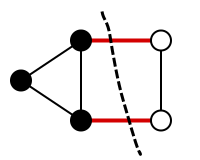
\includegraphics[width=.4\textwidth]{Min-cut.pdf}}
            \hspace{1em}
            \subfloat[Maximum Cut]{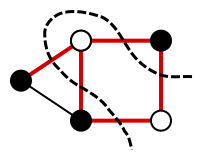
\includegraphics[width=.47\textwidth]{Max-cut.pdf}}
        \end{center}
    \end{figure}
\end{minipage}



\begin{minipage}{.55\linewidth}
    \theo{https://en.wikipedia.org/wiki/Prufer_sequence}
    {Prufer sequence}{
        Consider a labeled tree $ T $ with vertices's $ \{1, 2, ..., n\} $. At
        step $ i $, remove the leaf with the smallest label and set the $ i $th
        element of the \textit{Prüfer sequence} to be the label of this leaf's
        neighbour. Prove that a Prüfer sequence of length $ n-2 $ defines a Tree
        with length $ n $.

    }
\end{minipage}\hfill%
\begin{minipage}{.45\linewidth}
    \figdf{.4}{prufer_code_example}{${4,4,4,5}$}
\end{minipage}




\prob{https://artofproblemsolving.com/community/c6h5976p20088}
{German TST 2004 E7P3}{M}{
    We consider graphs with vertices colored black or white. ``Switching" a
    vertex means: coloring it black if it was formerly white, and coloring it
    white if it was formerly black.\\

    Consider a finite graph with all vertices colored white. Now, we can do the
    following operation: Switch a vertex and simultaneously switch all of its
    neighbours (i. e. all vertices connected to this vertex by an edge). Can we,
    just by performing this operation several times, obtain a graph with all
    vertices colored black?
}\label{problem:induction_type1_30}


\solu{A classical example of creating complex moves from counter cases.}


\prob{https://artofproblemsolving.com/community/c6h589936p3493453}
{ARO 2014 P9.8}{H}{
    In a country of $ n $ cities, an express train runs both ways between any
    two cities. For any train, ticket prices either direction are equal, but
    for any different routes these prices are different. Prove that the
    traveler can select the starting city, leave it and go on, successively, $
    n-1 $ trains, such that each fare is smaller than that of the previous
    fare. (A traveler can enter the same city several times.)
}\label{tickets}


\prob{https://artofproblemsolving.com/community/c6h364267}
{Generalization}{H}{
    Let $ A $ be a set of $ n $ points in the space. From the family of all
    segments with endpoints in $ A $ , $ q $ segments have been selected and
    colored yellow. Suppose that all yellow segments are of different length.
    Prove that there exists a polygonal line composed of $ m $ yellow
    segments, where $ m\geq\frac{2q}{n} $ , arranged in order of increasing
    length.
}\label{problem:constructive_algo_9}\label{problem:swapping_4}

\solu{
    Make one person go to every node. Then let the two people on the two sides
    of the most expensive edge swap their position. This ensures that every
    edge was used exactly 2 times. Using PHP, we have the desired result.
    Another solution is by 
    \autoref{theorem:mirsky_theorem}.
}



\prob{}
{}{E}{
    Given a bipartite graph, prove that the minimum number of colors required
    to color the edges of the graph such that no node is adjacent to $ 2 $
    edges of same color is the maximum degree of the graph.
}\label{problem:bipartite_graph_3}


\prob{}
{}{E}{
    For every bipartite graph prove that it's edges can be bicolored so that each
    node is adjacent to atmost $ \ceil{\dfrac{deg}{2}} $ edges of  any color.
}\label{problem:bipartite_graph_4}


\solu{Using the main property of a bipartite graph.}


\solu{After finding the cycle solution, to optimize it, we recall that we can find a Eulerian Path (if it exists) in $ O(V+E) $. Now we want to make the graph have a Eulerian path, so we add a vertice to both sides of the graph, and join them with odd vertices from the other side.}



\prob{https://artofproblemsolving.com/community/c6h446932}
{Turkey National MO 2002 P3}{HM}{
    Graph Airlines $(GA)$ operates flights between some of the cities
    of the Republic of Graphia. There are at least three $GA$ flights from each
    city, and it is possible to travel from any city in Graphia to any city in
    Graphia using $GA$ flights. $GA$ decides to discontinue some of its flights.
    Show that this can be done in such a way that it is still possible to travel
    between any two cities using $GA$ flights, yet at least $2/9$ of the cities
    have only one flight.

    \textbf{\Share\color{probC}Simplified:} In a connected graph, every
    vertex has degree at least $3$. Prove that some edges can be deleted to
    turn that graph into a tree with at least $\frac{2}{9}$ leaves. 

    \textbf{\Share\color{probC}Better Approximation:} We can actually achieve
    $\frac{1}{4}$ with careful construction.

    \index[strat]{Construction!Turkey NMO 2002 P3}
    \index[strat]{Bounding!Cost function!Turkey NMO 2002 P3}
}

\begin{solution}[dgrozev]
    First we construct a spanning tree $T$ that maximizes the number of leaves,
    then we bound the number. We define $G(V, E), n = \left|V\right| $ with
    the usual notations.\\

    Let $f: V \to V$. We initialize the tree by selecting a vertex $v$ by
    random, and adding it to $T$. We inductively add the vertices according to
    the following priority checks:

    \begin{enumerate}[label=\textbf{\boxed{\arabic*.}}, itemsep=5pt]
        \item If there is a vertex $v\not \in T$ that is connected to $u\in T$
            such that $u$ is not a leaf, then add $v, uv$ to $T$.
        \item If $u\in T$ is a leaf and there are two $v_1, v_2$ not in $T$
            that are connected to $u$, add $v_1, v_2$ and $uv_1, uv_2$ to $T$.
        \item If $u\in T$ is a leaf, and there is a $v$ which has two
            neighbors outside of $T$, then add $v, uv$ to $T$, and let $f(u)=v$.
        \item If $u\in T$ is a leaf, there is a $v \not \in T$ which is
            connected to at most one vertex outside $T$, and connected to
            $u'\in T$, then add $v, uv$ to $T$ and let $f(u) = u'$.
    \end{enumerate}
    This algorithm will add all the vertices to the tree. We now need to bound
    the number of leaves.\\

    Let $n_1, n_2, n_3$ be the set of vertices that have $1, 2$ and more than
    $3$ neighbors respectively. Since $f$ is a injection from the set $n_2$ to
    either $n_1$ or $n_3$, we have since $n = n_1+n_2+n_3$,
    \[n_2 \le n_1 + n_3,\quad n_2 \le \frac{n}{2}\]
    Bounding the number of edges gives us:
    \[\begin{aligned}
        2n-2 &\ge n_1 + 2n_2 + 3n_3\\
             &= n_1 + 3(n-n_1) - n_2\\
             &\ge 3n - 2n_1 - \frac{n}{2}\\
        \implies n_1 &\ge \frac{n}{4}+1
    \end{aligned}\]
\end{solution}

\begin{solution}[\href{http://wwwmayr.in.tum.de/konferenzen/Jass08/courses/1/gravin/Gravin_Slides.pdf}{Paper}]
    The construction is the same as before. But we define a different cost
    fuction $f$ to bound our leaves count. Let $D(T)$ be the number of leaves in
    $T$ which doesn't have a neighbor outside of $T$. Let $L(T)$ be the number of
    all leaves, and $V(T)$ is the number of vertices of $T$. Then consider 
    \[\boxed{f(T) = 3L(T) + D(T) - V(T)}\] 
    We show that $f(T)$ is non decreasing in our construction. If it is, we
    will get by setting $f(T_0)$ for a one vertex and its neighbor tree $T_0$, 
    \[f(T) \ge f(T_0) \ge 3\times 3 +0 -4 = 5 \] 
    And since $D(T') = L(T')$ for a spanning tree $T'$, \[L(T') \ge \frac{N+5}{4}\] 
    We now check that for all of your steps in construction, $f(T)$ is non
    decreasing.
\end{solution}



\prob{https://artofproblemsolving.com/community/c6h100733p568964}{ISL 2005 C1}{E}{A house has an even number of lamps distributed among its rooms in such a way that there are at least three lamps in every room. Each lamp shares a switch with exactly one other lamp, not necessarily from the same room. Each change in the switch shared by two lamps changes their states simultaneously. Prove that for every initial state of the lamps there exists a sequence of changes in some of the switches at the end of which each room contains lamps which are on as well as lamps which are off.}\label{problem:divide_and_conquer_4}\label{problem:induction_type1_10}



\prob{https://artofproblemsolving.com/community/c6h597130p3543398}{ISL 2013 C3}{M}{A crazy physicist discovered a new kind of particle which he called an $ i $ -mon, after some of them mysteriously appeared in his lab. Some pairs of $ i $ -mons in the lab can be entangled, and each $ i $ -mon can participate in many entanglement relations. The physicist has found a way to perform the following two kinds of operations with these particles, one operation at a time.

    \begin{enumerate}

        \item If some $ i $ -mon is entangled with an odd number of other $ i $ -mons in the lab, then the physicist can destroy it.

        \item At any moment, he may double the whole family of $ i $ -mons in the lab by creating a copy $ I' $ of each $ i $ -mon $ I $. During this procedure, the two copies $ I' $ and $ J' $ become entangled if and only if the original $ i $ -mons $ I $ and $ J $ are entangled, and each copy $ I' $ becomes entangled with its original $ i $ -mon $ I $ ; no other entanglements occur or disappear at this moment.

    \end{enumerate}

    Prove that the physicist may apply a sequence of much operations resulting in a family of $ i $ -mons, no two of which are entangled.
}\label{problem:induction_type1_9}


\solu{As there are an integer number of $ i $ -mons, it is quite natural to use induction. We try to find an algorithm to reduce the number of particles.

Another way to do this is to consider the chromatic number of the graph. If we can show that this number reduces after some move, then we are done by induction.}



\prob{https://artofproblemsolving.com/community/c6h104152p586762}{ISL 2005 C2}{E}{A forest consists of rooted (i. e. oriented) trees. Each vertex of the forest is either a leaf or has two successors. A vertex $ v $ is called an extended successor of a vertex $ u $ if there is a chain of vertices's $ u_{0}=u , u_{1}, u_{2} \dots u_{t-1} , u_{t}=v $ with $ t>0 $ such that the vertex $ u_{i+1} $ is a successor of the vertex $ u_{i} $ for every integer $ i $ with $ 0\leq i\leq t-1 $.\\

    Let $ k $ be a nonnegative integer. A vertex is called dynastic if it has two successors and each of these successors has at least $ k $ extended successors.\\

Prove that if the forest has $ n $ vertices, then there are at most $ \frac{n}{k+2} $ dynastic vertices.}\label{problem:induction_type1_8}

\solu{Trying to apply induction, we realize the bound is very loosy. That's why when we try to add in the inductive step, the value becomes larger than the bound. To stop that overflow, we tighten the bound.}

\solu{The second and dummy approach is to first doing some smaller cases, finding small infos, taking the root, seeing that the bound doesnt work, but it would work if one of the successors of the root would have exactly or less than $ 2k+3 $ successors. As we can't always guarantee that, we look for such a vertex with $ 2k+3 $ successors. We do some work with it and by induction its done.}



\prob{https://artofproblemsolving.com/community/c6h1441121p8200413}{All Russia 2017 9.1}{E}{In a country some cities are connected by oneway flights (There are no more then one flight between two cities). City $ A $ called "available" for city $ B $ , if there is flight from $ B $ to $ A $ , maybe with some transfers. It is known, that for every 2 cities $ P $ and $ Q $ exist city $ R $ , such that $ P $ and $ Q $ are available from $ R $. Prove, that exist city $ A $ , such that every city is available for $ A $.}\label{problem:induction_type1_17}



\prob{www.google.com}{Jacob Tsimerman Induction}{E}{There are $ 2010 $ ninjas in the village of Konoha (what? Ninjas are cool.) Certain ninjas are friends, but it is known that there do not exist $ 3 $ ninjas such that they are all pairwise friends. Find the maximum possible number of pairs of friends.(If ninja $ A $ is friends with ninja $ B $ , then ninja $ B $ is also friends with ninja $ A $.)}\label{problem:induction_type1_16}


\prob{https://artofproblemsolving.com/community/c6h420430p2374818}{USA TST 2011 D3P2}{M}{Let $n \geq 1$ be an integer, and let $S$ be a set of integer pairs $(a,b)$ with $1 \leq a < b \leq 2^n$. Assume $|S| > n \cdot 2^{n+1}$. Prove that there exists four integers $a < b < c < d$ such that $S$ contains all three pairs $(a,c)$, $(b,d)$ and $(a,d)$.}\label{problem:induction_type1_19}

\solu{Using Induction to the first and last half of the set $ S $ shows us the \hrf{finding_the_tough_nut}{hardest part} of the problem. Then ordering the left and right elements with some sort of hierarchy is all the work left to do.}




\prob{https://artofproblemsolving.com/community/c6h1480703p8639274}{ISL 2016 C6}{H}{There are $ n \geq 3 $ islands in a city. Initially, the ferry company offers some routes between some pairs of islands so that it is impossible to divide the islands into two groups such that no two islands in different groups are connected by a ferry route.\\

    After each year, the ferry company will close a ferry route between some two islands $ X $ and $ Y $. At the same time, in order to maintain its service, the company will open new routes according to the following rule: for any island which is connected to a ferry route to exactly one of $ X $ and $ Y $, a new route between this island and the other of $ X $ and $ Y $ is added.\\

Suppose at any moment, if we partition all islands into two nonempty groups in any way, then it is known that the ferry company will close a certain route connecting two islands from the two groups after some years. Prove that after some years there will be an island which is connected to all other islands by ferry routes.}\label{problem:induction_type1_11}

\solu{It is only natural to use induction on this kinda problems. After some trying, we see that if we remove $ 1 $ node, We get to nowhere, but if we remove $ 2 $ nodes, we get something interesting. So now focus on those two nodes and the rest of the nodes separately. Its not hard from there.}

\solu{As it seems, the separation of the graph was the main observation. We can call this trick \hl{Bringing Order in the Chaos}.}



\prob{https://artofproblemsolving.com/community/c6h535003p3067563}{ARO 2013 P9.5}{M (8/10)}{$ 2n $ real numbers with a positive sum are aligned in a circle. For each of the numbers, we can see there are two sets of $ n $ numbers such that this number is on the end. Prove that at least one of the numbers has a positive sum for both of these two sets.}\label{problem:graph_representation_4}\label{problem:minus_constant_2}

\solu{Since there is nothing specfic about the sum, we may safely assume that it is $ 0 $, because (1) probably it works, and (2) it makes things more convenient. How we do that? we decrease every number by the average.\\

    Now, Consider every block of $ n $ consecutive blockes of numbers. When are two blocks connected? When they share the same end. What if we consider them as vertices, and this ``connectivity'' as edges? We see that cycles pop out.\\

And we make use of the fact that our sum is $ 0 $. So signs are sure to bet flipped at the opposite side, and there are odd and even -ness in cycles that we can use.}




\prob{https://artofproblemsolving.com/community/c6h420424p2374799}{USA TST 2011 P2}{HM (9/10)}{In the nation of Onewaynia, certain pairs of cities are connected by roads. Every road connects exactly two cities (roads are allowed to cross each other, e.g., via bridges). Some roads have a traffic capacity of 1 unit and other roads have a traffic capacity of $ 2 $ units. However, on every road, traffic is only allowed to travel in one direction. It is known that for every city, the sum of the capacities of the roads connected to it is always odd. The transportation minister needs to assign a direction to every road. Prove that he can do it in such a way that for every city, the difference between the sum of the capacities of roads entering the city and the sum of the capacities of roads leaving the city is always exactly one.}\label{problem:divide_and_conquer_1}\label{problem:induction_type2_3}

\solu{As there are two types of subgraph, $ 1 $ -type and $ 2 $ -type. By some work-arounds, we see that we have to work distinctly in both types of graphs. Firstly, if we work in type- $ 1 $ , we see after making a path from node $ x, y $ , the degrees of $ x, y $ will be $ \{1, -1\} $ and the degrees of other nodes on the path will be the same. After that, we make every nodes have degree either $ \{1, -1\} $. So after this operation we remove the $ 1 $ -edges. Now, when dealing with the type- $ 2 $ sub-graph. Start over from zero, we see that when making a path between nodes $ x, y $ the degree of those two changes parity, and other nodes on the path stays the same. So select two odd nodes.... }

\solu{Dealing with two different kind of edges simultaneously is messy, so we work with graph $ 1 $ and graph $ 2 $ differently. Now on both graphs, we can remove cycles. And in graph $ 2 $ , we see that we can remove any big paths if there is a edge $ 1 $ joining the two endpoints. Since if the new graph works then the previous graph works too. [Several cases to show here] And if there is no edge joining the two endpoints, replace the path by joining the two endpoints by a edge $ 2 $.\\

Now there are only edge $ 1 $ s, and lone edge $ 2 $ s. Now dividing the graph $ 1 $ into paths of edge $ 1 $ , and dealing with several small cases, we are done.}



\prob{https://artofproblemsolving.com/community/c6h276187p1494557}{Iran TST 2009 P6}{E-M (9/10)}{We have a closed path that goes from one vertex to another neighboring vertex, on the vertices of a $ n\times n$ square which pass throgugh each vertex exactly once. Prove that we have two adjacent vertices such that if we cut the path at these two points then the length of each open paths is at least $ n^2/4 $.}

\solu{Draw a path, doesn't it look like a snake? Now can we relate the area of the tiled path with its perimeter? If we could do that, we would be able to replace two neighboring vertices by an edge inside the path, which seems to make the problem simpler.}



\prob{https://math.stackexchange.com/questions/1439430/algorithm-to-uniquely-determine-a-number-using-two-adjacent-digits}{OC Chap2 P2}{M (6/10)}{Arutyun and Amayak perform a magic trick as follows. A spectator writes down on a board a sequence of $ N $ (decimal) digits. Amayak covers two adjacent digits by a black disc. Then Arutyun comes and says both closed digits (and their order). For which minimal $ N $ can this trick always work? NOTE: Arutyun and Amayak have a strategy determined beforehand.}\label{problem:bijection_2}\label{problem:hall_marriage_1}

\solu{We have to actually find a bijection between all of the combinations the spectator can create, and all of the combinations that Arutyun might see when he comes back. Which tells us to use ``Perfect Matching" tricks.}

\solu{Existential proof: for this trick to always work, they have to make a bijection from a set of $ N $ digits with two covered, to an unique set of $ N $ digits. Consider a bijection from the set of $ 0-9 $ strings with length $ N $ to the set of $ 0-9 $ strings with length $ N $ with $ 2 $ adjacent digits unknown. There exist a bijection iff the two sets satisfy Hall's Marriage Theorem. By double counting we get the value of $ N $ from here.}



\prob{}{Simurgh 2019 P3}{E}{Call a graph \textit{symmetric}, if one can put its vertices on the plane such that it becomes symmetric wrt a line (which doesn't pass through any vertex). Find the minimum value of $ k $ such that (the edges of) every graph on $ 100 $ vertices, can be decomposed into $ k $ symmetric subgraph.}



\prob{https://artofproblemsolving.com/community/c6h2019175p14186360}
{RMM 2020 P3}{MH}{
    Let $n\ge 3$ be an integer. In a country there are $n$ airports and $n$
    airlines operating two-way flights. For each airline, there is an odd
    integer $m\ge 3$, and $m$ distinct airports $c_1, \dots, c_m$, where the
    flights offered by the airline are exactly those between the following
    pairs of airports: $c_1$ and $c_2$; $c_2$ and $c_3$; $\dots$ ; $c_{m-1}$
    and $c_m$; $c_m$ and $c_1$.

    Prove that there is a closed route consisting of an odd number of flights
    where no two flights are operated by the same airline.

    \index[strat]{Induction!Special!RMM 2020 P3}
    \index[strat]{Local!Add One by One!RMM 2020 P3}
    \index[strat]{Graph!Hall Marriage!RMM 2020 P3}
    \index[strat]{Graph!Bipartite!RMM 2020 P3}
}

\solu{[Weird Induction]
    Fix one vertice, merge all neighbors with it that has a unique airline between them.
}

\solu{[Element of Time]
    Add one edge from each cycle one at a time, without creating a cycle. Our objective is to show that when we reach the maximum stage where one edge creates a cycle, that cycle is of odd length.
}
